{ }%  A simple AAU report template.
%  2015-05-08 v. 1.2.0
%  Copyright 2010-2015 by Jesper Kjær Nielsen <jkn@es.aau.dk>
%
%  This is free software: you can redistribute it and/or modify
%  it under the terms of the GNU General Public License as published by
%  the Free Software Foundation, either version 3 of the License, or
%  (at your option) any later version.
%
%  This is distributed in the hope that it will be useful,
%  but WITHOUT ANY WARRANTY; without even the implied warranty of
%  MERCHANTABILITY or FITNESS FOR A PARTICULAR PURPOSE.  See the
%  GNU General Public License for more details.
%
%  You can find the GNU General Public License at <http://www.gnu.org/licenses/>.
%
%  A simple AAU report template.
%  2015-05-08 v. 1.2.0
%  Copyright 2010-2015 by Jesper Kjær Nielsen <jkn@es.aau.dk>
%
%  This is free software: you can redistribute it and/or modify
%  it under the terms of the GNU General Public License as published by
%  the Free Software Foundation, either version 3 of the License, or
%  (at your option) any later version.
%
%  This is distributed in the hope that it will be useful,
%  but WITHOUT ANY WARRANTY; without even the implied warranty of
%  MERCHANTABILITY or FITNESS FOR A PARTICULAR PURPOSE.  See the
%  GNU General Public License for more details.
%
%  You can find the GNU General Public License at <http://www.gnu.org/licenses/>.
%
\documentclass[12pt,twoside,a4paper,openright]{report}
%%%%%%%%%%%%%%%%%%%%%%%%%%%%%%%%%%%%%%%%%%%%%%%%
% Language, Encoding and Fonts
% http://en.wikibooks.org/wiki/LaTeX/Internationalization
%%%%%%%%%%%%%%%%%%%%%%%%%%%%%%%%%%%%%%%%%%%%%%%%
% Select encoding of your inputs. Depends on
% your operating system and its default input
% encoding. Typically, you should use
%   Linux  : utf8 (most modern Linux distributions)
%            latin1
%   Windows: ansinew
%            latin1 (works in most cases)
%   Mac    : applemac
% Notice that you can manually change the input
% encoding of your files by selecting "save as"
% an select the desired input encoding.
\usepackage[utf8]{inputenc}
% Make latex understand and use the typographic
% rules of the language used in the document.
\usepackage[danish]{babel}
\usepackage[footnote,mode=multiuser,draft,danish,silent,nomargin]{fixme}
% Use the palatino font
\usepackage[sc]{mathpazo}
\linespread{1.35}         % Palatino needs more leading (space between lines)
% Choose the font encoding
\usepackage[T1]{fontenc}
%%%%%%%%%%%%%%%%%%%%%%%%%%%%%%%%%%%%%%%%%%%%%%%%
% Graphics and Tables
% http://en.wikibooks.org/wiki/LaTeX/Importing_Graphics
% http://en.wikibooks.org/wiki/LaTeX/Tables
% http://en.wikibooks.org/wiki/LaTeX/Colors
%%%%%%%%%%%%%%%%%%%%%%%%%%%%%%%%%%%%%%%%%%%%%%%%
% load a colour package
\usepackage{xcolor}
\definecolor{aaublue}{RGB}{33,26,82}% dark blue
% The standard graphics inclusion package
\usepackage{graphicx}
% Set up how figure and table captions are displayed
\usepackage{caption}
\captionsetup{%
  font=footnotesize,% set font size to footnotesize
  labelfont=bf % bold label (e.g., Figure 3.2) font
}
% Make the standard latex tables look so much better
\usepackage{array,booktabs}
% Enable the use of frames around, e.g., theorems
% The framed package is used in the example environment
\usepackage{framed}
\usepackage{adjustbox}   
  

%%%%%%%%%%%%%%%%%%%%%%%%%%%%%%%%%%%%%%%%%%%%%%%%
% Mathematics
% http://en.wikibooks.org/wiki/LaTeX/Mathematics
%%%%%%%%%%%%%%%%%%%%%%%%%%%%%%%%%%%%%%%%%%%%%%%%
% Defines new environments such as equation,
% align and split
\usepackage{amsmath}
% Adds new math symbols
\usepackage{amssymb}
% Use theorems in your document
% The ntheorem package is also used for the example environment
% When using thmmarks, amsmath must be an option as well. Otherwise \eqref doesn't work anymore.
\usepackage[framed,amsmath,thmmarks]{ntheorem}

%%%%%%%%%%%%%%%%%%%%%%%%%%%%%%%%%%%%%%%%%%%%%%%%
% Page Layout
% http://en.wikibooks.org/wiki/LaTeX/Page_Layout
%%%%%%%%%%%%%%%%%%%%%%%%%%%%%%%%%%%%%%%%%%%%%%%%
% Change margins, papersize, etc of the document
\usepackage[
  inner=28mm,% left margin on an odd page
  outer=41mm,% right margin on an odd page
  ]{geometry}
% Modify how \chapter, \section, etc. look
% The titlesec package is very configureable
\usepackage{titlesec}
\titleformat{\chapter}[display]{\normalfont\huge\bfseries}{\chaptertitlename\ \thechapter}{20pt}{\Huge}
\titleformat*{\section}{\normalfont\Large\bfseries}
\titleformat*{\subsection}{\normalfont\large\bfseries}
\titleformat*{\subsubsection}{\normalfont\normalsize\bfseries}
%\titleformat*{\paragraph}{\normalfont\normalsize\bfseries}
%\titleformat*{\subparagraph}{\normalfont\normalsize\bfseries}

% Clear empty pages between chapters
\let\origdoublepage\cleardoublepage
\newcommand{\clearemptydoublepage}{%
  \clearpage
  {\pagestyle{empty}\origdoublepage}%
}
\let\cleardoublepage\clearemptydoublepage

% Change the headers and footers
\usepackage{fancyhdr}
\pagestyle{fancy}
\fancyhf{} %delete everything
\renewcommand{\headrulewidth}{0pt} %remove the horizontal line in the header
\fancyhead[RE]{\small\nouppercase\leftmark} %even page - chapter title
\fancyhead[LO]{\small\nouppercase\rightmark} %uneven page - section title
\fancyhead[LE,RO]{\thepage} %page number on all pages
% Do not stretch the content of a page. Instead,
% insert white space at the bottom of the page
\raggedbottom
% Enable arithmetics with length. Useful when
% typesetting the layout.
\usepackage{calc}

%%%%%%%%%%%%%%%%%%%%%%%%%%%%%%%%%%%%%%%%%%%%%%%%
% Bibliography
% http://en.wikibooks.org/wiki/LaTeX/Bibliography_Management
%%%%%%%%%%%%%%%%%%%%%%%%%%%%%%%%%%%%%%%%%%%%%%%%
\usepackage[backend=biber,
  bibencoding=utf8,
  style=authoryear,
  ]{biblatex}
\usepackage{filecontents}
\addbibresource{bib/mybib.bib}

%%%%%%%%%%%%%%%%%%%%%%%%%%%%%%%%%%%%%%%%%%%%%%%%
% Misc
%%%%%%%%%%%%%%%%%%%%%%%%%%%%%%%%%%%%%%%%%%%%%%%%
% Add bibliography and index to the table of
% contents
\usepackage[nottoc]{tocbibind}
% Add the command \pageref{LastPage} which refers to the
% page number of the last page
\usepackage{lastpage}
% Add todo notes in the margin of the document
\usepackage[
%  disable, %turn off todonotes
  colorinlistoftodos, %enable a coloured square in the list of todos
  textwidth=\marginparwidth, %set the width of the todonotes
  textsize=scriptsize, %size of the text in the todonotes
  ]{todonotes}

%%%%%%%%%%%%%%%%%%%%%%%%%%%%%%%%%%%%%%%%%%%%%%%%
% Hyperlinks
% http://en.wikibooks.org/wiki/LaTeX/Hyperlinks
%%%%%%%%%%%%%%%%%%%%%%%%%%%%%%%%%%%%%%%%%%%%%%%%
% Enable hyperlinks and insert info into the pdf
% file. Hypperref should be loaded as one of the
% last packages
\usepackage[T1]{fontenc}
\usepackage{mwe}    % loads »blindtext« and »graphicx«
\usepackage{subfig}



\usepackage{hyperref}
\hypersetup{%
	pdfpagelabels=true,%
	plainpages=false,%
	pdfauthor={Author(s)},%
	pdftitle={Title},%
	pdfsubject={Subject},%
	bookmarksnumbered=true,%
	colorlinks=false,%
	citecolor=black,%
	filecolor=black,%
	linkcolor=black,% you should probably change this to black before printing
	urlcolor=black,%
	pdfstartview=FitH%
}
\usepackage{cleveref} 
% package inclusion and set up of the document
% see, e.g., http://en.wikibooks.org/wiki/LaTeX/Formatting#Hyphenation
% for more information on word hyphenation
\hyphenation{ex-am-ple hy-phen-a-tion short}
\hyphenation{long la-tex}
%
%  A simple AAU report template.
%  2015-05-08 v. 1.2.0
%  Copyright 2010-2015 by Jesper Kjær Nielsen <jkn@es.aau.dk>
%
%  This is free software: you can redistribute it and/or modify
%  it under the terms of the GNU General Public License as published by
%  the Free Software Foundation, either version 3 of the License, or
%  (at your option) any later version.
%
%  This is distributed in the hope that it will be useful,
%  but WITHOUT ANY WARRANTY; without even the implied warranty of
%  MERCHANTABILITY or FITNESS FOR A PARTICULAR PURPOSE.  See the
%  GNU General Public License for more details.
%
%  You can find the GNU General Public License at <http://www.gnu.org/licenses/>.
%
%
%
% see, e.g., http://en.wikibooks.org/wiki/LaTeX/Customizing_LaTeX#New_commands
% for more information on how to create macros

%%%%%%%%%%%%%%%%%%%%%%%%%%%%%%%%%%%%%%%%%%%%%%%%
% Macros for the titlepage
%%%%%%%%%%%%%%%%%%%%%%%%%%%%%%%%%%%%%%%%%%%%%%%%
%Creates the aau titlepage
\newcommand{\aautitlepage}[3]{%
  {
    %set up various length
    \ifx\titlepageleftcolumnwidth\undefined
      \newlength{\titlepageleftcolumnwidth}
      \newlength{\titlepagerightcolumnwidth}
    \fi
    \setlength{\titlepageleftcolumnwidth}{0.5\textwidth-\tabcolsep}
    \setlength{\titlepagerightcolumnwidth}{\textwidth-2\tabcolsep-\titlepageleftcolumnwidth}
    %create title page
    \thispagestyle{empty}
    \noindent%
    \begin{tabular}{@{}ll@{}}
      \parbox{\titlepageleftcolumnwidth}{
        \iflanguage{danish}{%
          
\includegraphics[width=\titlepageleftcolumnwidth]{figures/aau_logo_da}
        }{%
          
\includegraphics[width=\titlepageleftcolumnwidth]{figures/aau_logo_en}
        }
      } &
      \parbox{\titlepagerightcolumnwidth}{\raggedleft\sf\small
        #2
      }\bigskip\\
       #1 &
      \parbox[t]{\titlepagerightcolumnwidth}{%
      \textbf{Abstract:}\bigskip\par
        \fbox{\parbox{\titlepagerightcolumnwidth-2\fboxsep-2\fboxrule}{%
          #3
        }}
      }\\
    \end{tabular}
    \vfill
    \iflanguage{danish}{%
      \noindent{\footnotesize\emph{Rapportens indhold er frit tilgængeligt, men offentliggørelse (med kildeangivelse) må kun ske efter aftale med forfatterne.}}
    }{%
      \noindent{\footnotesize\emph{The content of this report is freely available, but publication (with reference) may only be pursued due to agreement with the author.}}
    }
    \clearpage
  }
}

%Create english project info
\newcommand{\englishprojectinfo}[8]{%
  \parbox[t]{\titlepageleftcolumnwidth}{
    \textbf{Title:}\\ #1\bigskip\par
    \textbf{Theme:}\\ #2\bigskip\par
    \textbf{Project Period:}\\ #3\bigskip\par
    \textbf{Project Group:}\\ #4\bigskip\par
    \textbf{Participant(s):}\\ #5\bigskip\par
    \textbf{Supervisor(s):}\\ #6\bigskip\par
    \textbf{Copies:} #7\bigskip\par
    \textbf{Page Numbers:} \pageref{LastPage}\bigskip\par
    \textbf{Date of Completion:}\\ #8
  }
}

%Create danish project info
\newcommand{\danishprojectinfo}[8]{%
  \parbox[t]{\titlepageleftcolumnwidth}{
    \textbf{Titel:}\\ #1\bigskip\par
    \textbf{Tema:}\\ #2\bigskip\par
    \textbf{Projektperiode:}\\ #3\bigskip\par
    \textbf{Projektgruppe:}\\ #4\bigskip\par
    \textbf{Deltager(e):}\\ #5\bigskip\par
    \textbf{Vejleder(e):}\\ #6\bigskip\par
    \textbf{Oplagstal:} #7\bigskip\par
    \textbf{Sidetal:} \pageref{LastPage}\bigskip\par
    \textbf{Afleveringsdato:}\\ #8
  }
}

%%%%%%%%%%%%%%%%%%%%%%%%%%%%%%%%%%%%%%%%%%%%%%%%
% An example environment
%%%%%%%%%%%%%%%%%%%%%%%%%%%%%%%%%%%%%%%%%%%%%%%%
\theoremheaderfont{\normalfont\bfseries}
\theorembodyfont{\normalfont}
\theoremstyle{break}
\def\theoremframecommand{{\color{gray!50}\vrule width 5pt \hspace{5pt}}}
\newshadedtheorem{exa}{Example}[chapter]
\newenvironment{example}[1]{%
		\begin{exa}[#1]
}{%
		\end{exa}
}
% my new macros

\begin{document}
%frontmatter
\pagestyle{empty} %disable headers and footers
\pagenumbering{roman} %use roman page numbering in the frontmatter
%  A simple AAU report template.
%  2015-05-08 v. 1.2.0
%  Copyright 2010-2015 by Jesper Kjær Nielsen <jkn@es.aau.dk>
%
%  This is free software: you can redistribute it and/or modify
%  it under the terms of the GNU General Public License as published by
%  the Free Software Foundation, either version 3 of the License, or
%  (at your option) any later version.
%
%  This is distributed in the hope that it will be useful,
%  but WITHOUT ANY WARRANTY; without even the implied warranty of
%  MERCHANTABILITY or FITNESS FOR A PARTICULAR PURPOSE.  See the
%  GNU General Public License for more details.
%
%  You can find the GNU General Public License at <http://www.gnu.org/licenses/>.
%
\pdfbookmark[0]{Front page}{label:frontpage}%
%mainfile: ../master.tex
\begin{titlepage}
	\begin{center}
		\newcommand{\HRule}{\rule{\linewidth}{0.5mm}}

		% Upper part of the page. The '~' is needed because \\
		% only works if a paragraph has started.
		
\includegraphics[width=0.5\textwidth]{figures/aau_logo_en.pdf}~\\[1cm]

		%\textsc{\LARGE Aalborg University}\\[1.5cm]

		%\textsc{\Large Project Report}\\[0.5cm]

		% Title
		\HRule \\[0.4cm]
		{ \huge Not done yet\\[0.4cm]
			\large \textsc{P1}}

		\HRule \\[1.5cm]

		% Author and supervisor
		\begin{minipage}{0.4\textwidth}
			\begin{flushleft} \large
				\emph{Projekt Gruppe}\\
				\textsc{B2-23}
			\end{flushleft}
		\end{minipage}
		\begin{minipage}{0.4\textwidth}
			\begin{flushright} \large
				\emph{Vejleder} \\
				\textsc{Søren Dam Nielsen}
				\emph{Kontekstuel Vejleder} \\
				\textsc{Niels Agerholm}
			\end{flushright}
		\end{minipage}

		\vfill

		% Bottom of the page
		{\large 18. Maj 2016}

	\end{center}
\end{titlepage}

\clearpage

\thispagestyle{empty}
{\small
\strut\vfill % push the content to the bottom of the page
\noindent Aalborg University 2016\par
\vspace{0.2cm}
\noindent

%\pdfbookmark[0]{English title page}{label:titlepage_en}
%\aautitlepage{%
 % \englishprojectinfo{
  %  Project Title %title
  %}{%
  %  Scientific Theme %theme
  %}{%
   % Fall Semester 2010 %project period
  %}{%
  %  XXX % project group
 % }{%
    %list of group members
   % Author 1\\
    %Author 2\\
    %Author 3
  %}{%
    %list of supervisors
   % Supervisor 1\\
    %Supervisor 2
  %}{%
   % 1 % number of printed copies
  %}{%
   % \today % date of completion
 % }%
%}{%department and address
 % \textbf{Electronics and IT}\\
  %Aalborg University\\
 % \href{http://www.aau.dk}{http://www.aau.dk}
%}{% the abstract
 % Here is the abstract
%}

%\cleardoublepage
%{\selectlanguage{danish}
%\pdfbookmark[0]{Danish title page}{label:titlepage_da}
%\aautitlepage{%
  %\danishprojectinfo{
   % Rapportens titel %title
  %}{%
   % Semestertema %theme
  %}{%
   % Efterårssemestret 2015 %project period
  %}{%
   % A405a % project group
 % }{%
    %list of group members
  %  	Abdul Massir Qauomi\\
   % 	Bjørn Carlson\\
    %	Fatimah Daoud\\
    %	Morten Bache Jacobsen\\
    %	Rasmus Steffensen\\
    %	Rong Liu
  %}{%
    %list of supervisors
   % Katrine Rabjerg Meltofte

  %}{
    1 % number of printed copies
  %}{%
    \today % date of completion
 % }%
%}{%department and address
  %\textbf{Elektronik og IT}\\
 % Aalborg Universitet\\
  %\href{http://www.aau.dk}{http://www.aau.dk}
%}{% the abstract
 % Her er resuméet
%}}
\markboth{Titlepage}{Titlepage} % Add to header

\begin{nopagebreak}
	{\begin{center}
			\begin{tabular*}{\textwidth}{@{}l@{\extracolsep{\fill}}r@{}}
				\multicolumn{2}{@{}l@{}}{
					\begin{minipage}[t]{1.0\textwidth}
						\vspace{0.3cm}
					\end{minipage}
				}\\
				\begin{minipage}[t]{0.49\textwidth}
					\textbf{Titel}\\
					Fundering af tilbygning af Strøybergs Palæ\\

					\textbf{Tema}\\
					???Virkelighed og modeller indenfor byggeri og anlæg\\

					\textbf{Projekt Periode}\\
					Forårs Semester 2016\\

					\textbf{Projekt Gruppe}\\
					B2-23\\

					\textbf{Forfattere}\\
					Abdul Massir Qauomi\\
					Alexander Schacht\\
					Emil Faber B.-S.\\
					Hussein Al-Ali\\
					Johnny Tuan N.\\
					Jonas Damsbo\\
          Mads Bjørndal N.\\


          \textbf{Vejleder} \\
          Søren Dam Nielsen \\
          \textbf{Kontekstuel Vejleder} \\
          Niels Agerholm


					\textbf{Kopier}\\
					2\\ % https://www.moodle.aau.dk/course/view.php?id=8838

					\textbf{Antal Sider}\\
					\pageref{LastPage}\\

				\end{minipage}
				&
				\begin{minipage}[t]{0.49\textwidth}
					\begin{flushright}
						
\includegraphics[height=3cm]{figures/aau_logo_en.pdf}\\
						\small \textbf{Byggeri og Anlæg 2. Semester} \\
						\small \textbf{INSTITUT FOR BYGGERI OG ANLÆG}\\
						\small Badehusvej 13 \\
						\small 9000 Aalborg\\
						\small \url{http://www.byggeri.aau.dk/}\\
						\bigskip
						\fbox{
							\parbox{\linewidth}{
								{\section{Synopsis}
\label{sec:synopsis}





{\tiny Dette projekt omhandler en vurdering af trygheden af trafikken i Nytorv/Østerågade området i Aalborg. Der er set på overvejelser omkring fodgængernes tryghed og sikkerhed i området.
\\
Der er blevet redegjort for områdets beliggenhed og struktur, samt om begrebet Shared Space. Her er der forklaret, hvilke årsager der kan være medvirkende til at tiltrække mange trafikanter.
\\
Områdets udseende er blevet diskuteret med henblik på Shared Space. Der er herunder set på sammenligninger, og folks færden i området.
\\
Der er lavet interviews af fodgængere, hvor der er set på deres opfattelse af trygheden i området. Herudover er interviewsene blevet udarbejdet for at få en forståelse for nogle generelle holdninger og trafikale problemer.
\\
Der er foretaget nogle observationer ved et fodgængerfelt i området, hvor fodgængernes sikkerhed i forhold til cyklisterne er diskuteret. Der er endvidere foretaget beregninger af TA-værdien og lavet adfærdsregistrering.
\\
Trafiktællinger er blevet foretaget, og der er blevet udarbejdet et flow kort over området. Herunder er der lavet beregninger af ÅDT.
\\
Forslag til løsninger, med henblik på de foretaget observationer, interviews og trafiktællinger, er blevet diskuteret, og områdets udseende er blevet perspektiveret.}

								}
							}}
						\end{flushright}
					\end{minipage}

					\\
				\end{tabular*}
			\end{center}
		}
	\end{nopagebreak}

\cleardoublepage
\pdfbookmark[0]{Contents}{label:contents}
\pagestyle{fancy} %enable headers and footers again
\tableofcontents
%\listoftodos
%\chapter*{Preface\markboth{Preface}{Preface}}\label{ch:preface}
%\addcontentsline{toc}{chapter}{Preface}
%Here is the preface. You should put your signatures at the end of the preface.

%\vspace{\baselineskip}\hfill Aalborg University, \today
%\vfill\noindent
%\begin{minipage}[b]{0.45\textwidth}
 %\centering
 %\rule{\textwidth}{0.5pt}\\
 % Author 1\\
 %{\footnotesize <username1@XX.aau.dk>}
%\end{minipage}
%\hfill
%\begin{minipage}[b]{0.45\textwidth}
 %\centering
 %\rule{\textwidth}{0.5pt}\\
 % Author 2\\
 %{\footnotesize <username2@XX.aau.dk>}
%\end{minipage}
%\vspace{3\baselineskip}
%\begin{center}
%\begin{minipage}[b]{0.45\textwidth}
 %\centering
 %\rule{\textwidth}{0.5pt}
 % Author 3\\
 %{\footnotesize <username3@XX.aau.dk>}
%\end{minipage}
%\end{center}
%mainfile: ../master.tex
\chapter*{Forord\markboth{Forord}{Forord}}\label{ch:forord}
\addcontentsline{toc}{chapter}{Forord}


\vspace{\baselineskip}\hfill Aalborg Universitet, 18. December 2015
\vfill
\newpage
\noindent
\\\\
\begin{minipage}[b]{0.45\textwidth}
	\centering
	\rule{\textwidth}{0.5pt}\\
	Abdul Massir Qauomi\\
	{\footnotesize <aqauom15@student.aau.dk>}
\end{minipage}
%
\hfill
%
\begin{minipage}[b]{0.45\textwidth}
	\centering
	\rule{\textwidth}{0.5pt}\\
	Alexander Schacht\\
	{\footnotesize <xxxx@student.aau.dk>}
\end{minipage}
%
\vspace{3\baselineskip}

\noindent
\begin{minipage}[b]{0.45\textwidth}
	\centering
	\rule{\textwidth}{0.5pt}\\
	Emil Faber B.-S.\\
	{\footnotesize <xxxx@student.aau.dk>}
\end{minipage}
%
\hfill
%
\begin{minipage}[b]{0.45\textwidth}
	\centering
	\rule{\textwidth}{0.5pt}\\
	Hussein Al-Ali\\
	{\footnotesize <XXXX@student.aau.dk>}
\end{minipage}
\vspace{3\baselineskip}

\noindent
\begin{minipage}[b]{0.45\textwidth}
	\centering
	\rule{\textwidth}{0.5pt}\\
	Johnny Tuan N.\\
	{\footnotesize <xxxx@student.aau.dk>}
\end{minipage}
%
\hfill
%
\begin{minipage}[b]{0.45\textwidth}
	\centering
	\rule{\textwidth}{0.5pt}\\
	Jonas Damsbo\\
	{\footnotesize <XXX@student.aau.dk>}
\end{minipage}

\hfill
%
\begin{minipage}[b]{0.45\textwidth}
	\centering
	\rule{\textwidth}{0.5pt}\\
	Mads Bjørndal N.\\
	{\footnotesize <XXXX@student.aau.dk>}
\end{minipage}
\vspace{3\baselineskip}


\vspace{3\baselineskip}

%\cleardoublepage
%mainmatter
\pagenumbering{arabic} %use arabic page numbering in the mainmatter
\input{sections/report/indledning/indledningmaster.tex}
%mainfile: master.tex
\chapter{Problemformulering}
\label{chap:problemformulering}
~\\\\
Det er interresant at se på, hvordan trafikken fungerer nede ved Nytorv/Østerågade området, i og med, at der færdes mange trafikanter, og det er et af de centrale steder i Aalborg by. De mange shoppingfaciliteter og cafémuligheder gør det til et attraktivt sted, især for fodgængere at færde sig i, og derfor er det især denne trafikantgruppe, der er i højsædet i dette projekt. Problemstillingerne er ikke store den dag i dag, men set i perspektivet af, at Aalborg har befolkningsvækst, kan der i fremtiden opstå store trafikale problemer i området. Det er derfor relevant at undersøge, hvilke konflikter, forbigående fodgængere og cyklister mener er til stede mellem dem og de andre trafikantgrupper.
Det er også interresant at se på om området fungerer som et Shared Space område eller noget helt andet.
Det leder efterfølgende til en masse ideer om en eller flere eventuelle løsninger på de trafikale problemer, der kan tænkes at være til stede i området, og dermed løse fremtidens trafikale problemstillinger. Det er især et fokus på en effektivisering af trafik flowet, der i dette projekt cirkuleres omkring. Udgangspunktet i projektet vil blive taget i følgende spørgsmål.
\\\\
Hvilke konflikter finder sted mellem cyklister og fodgængere på Nytorv/Østerågade?
\\
Hvordan kan et løsningsforslag løse de eventuelle konflikter?
\\
Hvordan kan der eventuelt skabes et bedre trafik flow ved området?
\\\\

\section{Afgrænsning}
\label{sec:afgraensning}

I dette projekt er der fokuseret på trafikkonflikter mellem cyklister og fodgængere på Nytorv/Østerågade i Aalborg. Fokuspunktet er fodgængernes tryghed overfor cyklisterne og bilerne. Der vil ikke blive fokuseret på buschauførrenes syn på sikkerheden eller dem der kører privatbiler, da de desuden er udelukket fra området. Der er blevet valgt i projektet at afgrænse sig til at lave kvalitative interviews af fodgængere og observationer af Nytorv. Desuden er der en afgrænsning i forhold til de forskellige trafikantgrupper, da der vil blive lavet interviews, udelukkende med forbipasserende som går eller cykler på Nytorv. Der vil blive undersøgt, om fodgængerne føler sig trygge, når de går på Nytorv/Østerågade i Aalborg. Der tages udgangspunkt i konflikter, der kan forekomme mellem cyklister og fodgængere, og hvordan der i området kan skabes et bedre trafik flow.

I undersøgelsen har projektet til formål at vurdere disse trafikkonflikter, og ved hjælp af de forskellige observationsmetoder og interviews, komme med et eller flere forslag til nogle konstruktive løsningsforslag, som kan forøge trygheden for cyklister samt fodgængere ved Nytorv/Østerågade området.

%master.tex
\chapter{Analyse}
\label{chap:analyse}


%\input{sections/report/analysedel/sharedspace.tex}
%\input{sections/report/analysedel/interviews.tex}
%\input{sections/report/analysedel/trafiktaellinger.tex}
%\input{sections/report/analysedel/resultateraftryghed.tex}

\section{Løsningforslag}


%\input{sections/report/losningforslag/cykelsti.tex}
%\input{report/losning/hvidfodgaengeroverfelt}
%\input{sections/report/losningforslag/rundkoersel.tex}
%\input{sections/report/losningforslag/bussluse.tex}

\chapter{Sonnenfelsplatz i byen Graz i Østrig kontra Nytorv/Østerågade i byen Aalborg i Danmark}
\label{chap:sonnenfelsplatz_i_byen_Graz_i_ostrig kontra_nytorv/osteraagade_i_byen_aalborg_i_danmark}

Den Østrigske by Graz renoverede i 2011 Sonnenfelsplatz til et Shared Space område. Sonnenfelsplatz er en central plads som har butikker og restauranter. Derudover ligger byens universitet campus lige i nærheden. \autocite{ssing2015}
I belastningsperioder har Sonnenfelsplatz i byen Graz i Østrig 15.000 køretøjer, 3.400 fodgængere og 640 cyklister i timen. I følge anvendelsen af Shared Space, anbefaler de at Shared Space bør anvendes ved trafikmængder på maks. 3.000- 4.000 motorkøretøjer/døgn, hvilket ikke er tilfældet i byen Graz i Østrig. \autocite{vejlednigomss2013}
Da køretøjerne skaber de fleste trafikbelastninger, og da vejoverfladen er skadet, og infrastrukturen under jorden har haft behov for renovering blev området lavet om. Herved blev Shared Space et mål for området, for at skabe en bebolig gade med frit kultur mobilitet, hvor der er plads til alle trafikanter. I den anledning er vejskilte og vejafmærkninger bevidst blevet valgt fra, da det vil få de forskellige trafikantgrupper til at integrere sig efter hinanden afhængigt af situationen i området. Dette kan også ses tydeligt på vejbanen.
På Sonnenfelsplatz er der ikke højdeforskel i vejen som afskiller kørertøjer fra fodgængere. Trafikanterne bliver opfordret til at dele og respekterer hinanden om pladsen. I midten af pladsen er der lavet en lille rundkørsel. Området anvender meget få skilte og vejmarkeringer, hvilket kan ses i området Sonnenfelsplatz, som ses på figur \cref{fig:cykelsti} på side \pageref{fig:cykelsti}. \autocite{SP2015}

\begin{figure}[htbp]
  \centering
  \begin{adjustbox}{max width=\textwidth}
    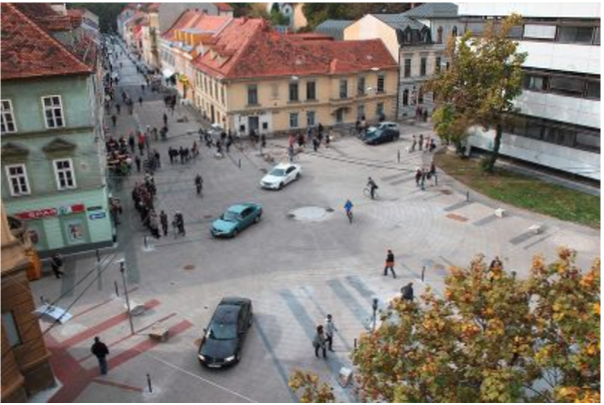
\includegraphics{figures/Billederogfigur/Perspektivering/en_andne_by.png}
 \end{adjustbox}
  \caption{Cykelsti \autocite{sonne}}
   \label{fig:cykelsti}
\end{figure}

~\\
I indledningen er Nytorv/Østerågade i byen Aalborg beskrevet som et samlingspunkt, hvor der på tilsvarende måde færdes mange mennesker og køretøjer. I området er der mange shopping- og cafémuligheder, derudover færdes der mange mennesker i området, som transportere sig med bus og på cykel. I følge trafiktællingerne der er foretaget i rapporten \cref{sub:trafiktaellinger} har Nytorv/Østerågade i byen Aalborg i Danmark et døgns trafik på 394 biler og der er 3.826 cykler på en november dag. I interviewet \cref{chap:interviews} mener flere af interviewpersoner, at bilerne og cyklisterne skaber utryghed for fodgængerne, hvilket giver årsag til, at der i rapporten fokuseres på at differentiere trafikantgrupperne. Det er blevet gjort ved at lave nogle forslag om at have en cykelbane i området, hvor cyklisterne kan cykle på deres egen bane, og en busluse for at udelukke bilerne fra området, hvilket kan ses på de nedenstående billeder.

~\\
Ligheden mellem området Sonnenfelsplatz i byen Graz og Nytorv/Østerågade i Aalborg er, at de to områder har nogle trafikantgrupper som deler kørerbanen. For Nytorvs/Østerågades tilfælde er der tale om fodgængere, cyklister, busser og erhvervsbiler for, og for Sonnenfelsplatz er det alle traffikantgrupperne der deler vejen.
~\\
Forskellen på de to områder er, at der er forbud for gennemkørsel af privatbiler på Nytorv/Østerågade, dog bliver færdselsloven ikke overholdt. Det er ikke tilfældet i Sonnenfelsplatz, da det er kørertøjerne der skaber de fleste trafikbelastninger. Ifølge døgns trafikken og blandt andet interviewpersonerne er det cyklisterne der skaber trafikbelastninger. Derudover bevæger området i Nytorv/Østerågade sig længere væk fra at være shared space og tættere på næsten at være en sivegade, da der blandt andet er højdeforskel i vejen som afskiller kørertøjer fra fodgængere. I Sonnenfelsplatz bevæger området sig tættere på at være Shared Space, da højdeforskellen på vejen ikke afskiller kørertøjer fra fodgængere.

\chapter{Diskussion}
\label{chap:diskussion}
For at kunne afgøre hvad eller hvilke eventuelle løsningsforslag, som løser rapportens undersøgte problemer bedst, er det væsentligt at se på fordele og ulemper ved de forskellige forslag. Ved at etablere en rundkørsel skabes, vil alle trafikantgrupper blive tvunget til at øge deres trafikale fokus, som konsekvens af rundkørslen. Samtidig må det forventes, at deres hastigheder må blive sænket en del. En af ulemperne ved at anlægge en rundkørsel vil på sigt blive en ringere offentlig transport i området, da det kan forsinke bustrafikken at føre dem gennem en rundkørsel på en trafikeret dag. En rundkørsel er særdeles effektiv at bruge som løsningsforslag et sted, hvor der er mange biler, som skal gennem et punkt. Eftersom det største problemfokus på Nytorv ikke er bilerne, men derimod cyklisterne, vil en rundkørsel muligvis gøre mere skade end gavn, hvis en sådan etablering blev en realitet. ~\\
Hvis der i stedet rettes fokus på løsningsforslaget med at anlægge en busgrav eller hæve-sænke pullert, er dette forslag, som det forrige, også fokuseret på bil problemet omkring Nytorv. Det ville afhjælpe problemet med de mange uvedkommende biler, der hver eneste dag kører ind i området, trods påbud, som tilsyneladende ikke har den ønskede virkning. En af fordelene bliver hermed, at Nytorv bliver helt fri for uvedkommende biler, og dette vil medvirkende til at skabe et mere forudsigeligt og måske mere trygt trafikmiljø. ~\\
Det sidste løsningsforslag beskæftiger sig med en anlægning af cykelbaner i hele området og omkring Nytorv. Fordelene er, at dette er med til at øge fokus på cyklisterne, og det giver et mere klart billede af, hvor cyklerne skal være på vejen. En af de overvejende ulemper er, at en cykelbane vil skabe gnidninger mellem cyklisterne og buspassagererne, når de skal af og på bussen. En cykelbane vil nemlig være etableret langs buslommen, og derved vil buspassagerende være nødsaget til at gå over cykelbanen. Det vil derfor være en nødvendighed, at cyklisterne er opmærksomme og holder tilbage for passagerende. ~\\
Da der i forvejen er et forholdsvis smalt fortov nogle steder nede ved Nytorv, bliver det ligeså svært at få plads til de eventuelle cykelbaner. De to første løsningsforslag har fokus på eventuelle bilproblemer, hvorimod det sidste løsningsforslag har til formål at afhjælpe cykelproblemer i trafikken. Eftersom det største trafikale problem nede ved Nytorv er mellem cyklister og fodgængere, er det oplagt at videreudvikle på ideen omkring en cykelbane.
~\\
I rapporten har den helt centrale problemstilling været, at undersøge trafikale problemer mellem fodgængere og cyklister ved fodgængerfeltet. Gennem de beregnede TA-værdier og de mange interviews, er der blevet vurderet, at der er et trafikalt problem netop på dette sted mellem cyklisterne og fodgængerne. Bilerne og busserne er gennem de foretagede interviews ikke blevet vurderet til at være et stort problem, og derfor er løsningsforslaget om cykelbanen valgt at blive diskuteret her, som den bedste løsning, for netop denne undersøgelse.
~\\
En etablering af en cykelbane vil have til formål at lede cyklisten inde for en afmærket sti, og på den måde fastholde cyklisten inden for afmærkningen Der vil herved blive formået at kontrollere cyklisternes kørebane og opretholde cyklistens fokus i selve kørebanen. Det formodes, at cyklisten vil få øje på en fodgængeren hurtigere, da der ikke er andre trafikanter cyklisten nu skal holde øje med. Det kan muligvis være med til, at der vil kunne observeres mange flere tidlige samspil end sene samspil ved fodgængeroverfeltet.. Et sådant formål, ville en etablering af en rundkørsel eller bussluse ikke opfylde. Set i et andet perspektiv, så kan det måske føre til flere kollisioner mellem fodgængere og cyklister, hvis cyklisten ser cykelbanen som sin helt egen bane. Der vil derfor være et dilemma, hvis der ikke bliver taget hensyn til de eventuelle passerende fodgængere eller biler, som svinger ind over cykelbanen. Derfor vil en cykelbane ikke være en endegyldig løsning på konflikterne ved fodgængerfeltet, da det kan tænkes, at der rent faktisk vil kunne opstå flere uheld end før. Men det er klart, at en cykelbane vil kunne guide cyklisterne, og have et bidrag til et mere trygt trafikmiljø på Nytorv/Østerågade området. Dog kan det diskuteres, om det er cyklisten eller fodgængeren, som vil føle sig mere tryg.

\chapter{Konklusion}
\label{chap:konklusion}
Det kan hermed konkluderes, at konflikterne mellem cyklister og fodgængere i og omkring området Nytorv/Østerågade er gensidige. Som det konkluderes i afsnittet om resultater af observation, er hovedparten af alle konflikter, som finder sted ved fodgængerfeltet på Østerågade er alvorlige. Dette konkluderes sådan, eftersom cyklisterne og fodgængerne kommer tæt på hinanden ved nogle bestemte hastigheder. Motivationen til at undersøge konflikter mellem cyklister og fodgængere kom fra interviewsene, og skabte en yderligere nysgerighed. Der er blevet observeret både tidlige og sene samspil, men dog flest sene samspil, som teoretisk indikerer, at området omkring fodgængerfeltet er et usikkert område for fodgængerne. De typer konflikter, der primært finder sted, som det også tidligere i rapporten er blevet defineret, er mellem cyklister og fodgængere, som er på kollisionskurs.~\\
 Yderligere kan vi sige, at dette underbygges i form af vores observationer og trafiktællinger, da vi i vores trafiktælling af trafikantgrupperne fandt frem til, at fodgængerfeltet på Østerågade var det mest befærdet sted for alle cyklister, fodgængere og billister i hele området. Ud fra denne opdagelse valgte vi derfor at sætte vores fokus på netop denne location under vores observationer. Om hvorvidt området er Shared Space eller ej vurderer vi, at det er en blanding af både et Shared Space område og en sivegade, da der er elementer af begge begreber i området.~\\
 Et løsningsforslag, som eksempelvis det forslag der kommer i rapporten vedrørende en cykelbane, vurderer vi til at have en sandsynlig mulighed for at kunne løse eventuelle konflikter mellem cyklister og fodgængere, da cyklerne bliver på denne måde mere synliggjorte i trafikområdet. For at skabe et bedre trafik flow, mener vi, at det er nødvendigt at lave ændringer i området. En eventuel ændring, som ville kunne have en markant effekt, og dermed give et bedre trafik flow, kunne være at etablere en cykelbane i hele området. Dette ville som tidligere skrevet øge fokus omkring, hvor cyklerne er, da de bliver henvist til at køre inden for de afmærkede cykelbaner. Dette kan dog også have en negativ effekt, da vi er bange for, at det kan få cyklisterne til at miste fokus på andre trafikkantgrupper, da de kun er nødsaget til at følge deres egen private bane.
 Projektetes formål, om at undersøge trygheden i området, er blevet undersøgt ved hjælp af sikkerhedsundersøgelser. Dette ligger til grund i, at tryghed ikke kan regnes på. I og med at den undersøgte sikkerhed ikke har været optimal ud fra vores beregninger, og trygheden ikke har været optimal ud fra de lavede interviews, vil der formodes at være en form for sammenhæng. Derfor er projektet mundet ud i et løsningsforslag til et mere sikkert trafikmiljø.

\printbibliography[heading=bibintoc]
\label{bib:mybiblio}
\appendix
\appendix
\label{appendix_start}
\chapter{Interviews}
  \label{chap:interviews}
Interview resultater med forbigående fodgængere og cyklister ved Nytorv/Østerågade i Aalborg I dette afsnit er 4 spørgsmål beskrevet, som blev stillet og svarerende fra 20 forbigående fodgængere og cykelister ved Nytorv/Østerågade, hvor de væsentlige svar er med i rapporten.
~\\
  \textbf{Spørgsmål 1.}
  Føler du dig tryg ved, at gå over fodgængerfeltet, når der er mange cyklister ude ved Nytorv/Østerågade i Aalborg?
~\\\\
  \textbf{Svar 1.} ~\\
 \emph{”Jeg føler mig tryg af, at gå over fodgængerfeltet, når der er mange cyklister. Jeg synes at de fleste holder pænt tilbage”.}
~\\\\
  \emph{”Jeg er Københavner, og jeg synes, at det er mere betryggende, at gå ude på strøget i København, der cykler ingen forbi, der er kun tværgående trafik. Jeg synes, at det er værre med bilerne, også må cyklisterne gerne være herude synes jeg.”}
~\\\\
  \emph{”Jeg bruger normalt lidt tid på, at se efter om cyklisterne har set mig eller om jeg selv skal stå tilbage, også går jeg over”}
~\\\\
\emph{” Jeg synes godt, at der kan være kaos herude nogle gange, og det er både cyklister, biler og busser der skaber den kaos.”}
~\\\\
  \emph{”Jeg føler mig tryg, da jeg tror at cyklisterne tænker, at jeg er gammel og de skal passe lidt på, men jeg træder aldrig ud uden at se mig for, jeg passer virkelig på.”}
~\\\\
  \emph{“Nej - holder øje til højre og venstre, og så kommer der nogle gange også en bil som ikke skal køre herinde.”}
~\\\\
  \emph{“Jeg føler mig tryg og cyklerne holder tilbage for en.”}
~\\\\
  \emph{“Nej - cyklerne holder ikke færdselsloven og holder ikke tilbage for fodgængerne.”}
~\\\\
  \emph{“Jeg føler mig tryg, når jeg går over vejen. En gang imellem ser man, at nogle stopper op og andre gør ikke, men jeg har ikke noget problem med det.”}
~\\\\
  \emph{“Ja det er jeg - de er gode til at holde tilbage.”}
~\\\\
  \emph{“Egentlig ikke - jeg synes, at cyklerne kommer meget uventet og meget hurtigt. Jeg holder utroligt meget øje.”}
~\\\\
\emph{“Nej egentlig ikke - de holder ikke tilbage - det er cyklerne- jeg er mere tryg ved bilerne.”}
~\\\\
\emph{“Ja det gør jeg faktisk - der er mange mennesker, men jeg synes ikke det er et problem.”}
~\\\\
  \emph{“Ikke altid - jeg er lige hoppet over for en cyklist.”}
~\\\\
  \emph{”Jeg bor lige herude. Man kan ikke gå og regne med at der ikke er andre end en selv herude, men jeg synes ikke engang at der er ret trafikeret, det kunne have været meget værre. Jeg synes at det er helt fint herude.”}
~\\\\
  \emph{“Cyklisterne kører sgu som en brækket arm, Så nej jeg føler mig ikke tryg.”}
~\\\\
  \textbf{Spørgsmål 2}
  ~\\
  Hvad er det, der gør dig utryg/tryg, når du går over fodgængerfeltet? og hvad er det vigtigste for dig, for at du føler dig tryg i et integreret trafikmiljø?
~\\
  \textbf{Svar 2} ~\\
\emph{“Noget mere overvågning, så biler der ikke skal køre derinde, ikke kan komme ind.”}
~\\\\
  \emph{”at vi fodgængere, cyklister og biler nærmest deler vejen, og at det ikke alle der tager hensyn til hinanden, vil føle mig mere tryg hvis vi var delt.”}
~\\\\
  \emph{“Her på Boulevarden lagde jeg mærke til at cyklisterne ikke kunne være der, så de måtte trække deres cykler på fortovet. De kunne slet ikke være der overhovedet.  Derfor stiller jeg min cykel i Arkaden og går hernede.”}
~\\\\
  \emph{“Jeg benytter mig af fodgængerovergangen, og det gør mig tryg.”}
~\\\\
  \emph{“At færdselsloven bliver overholdt.”}
~\\\\
  \emph{“Det må være det, men om morgenen så er der fart på her i området, altså mange folk cykler mod skoler, universitet og på arbejde. Men så længe at vi alle opmærksomme og buschaufførerne ved godt, at der er fodgængere her, så de er også opmærksomme, at området er gågade.”}
~\\\\
  \emph{“At folk viser hensyn til hinanden.”}
~\\\\
  \emph{“Folk holder automatisk tilbage - det gør de jo ikke.”}
~\\\\
  \emph{“At fodgængerfeltet er helligt og folk holder tilbage.”}
~\\\\
  \emph{“Det er at busserne og bilerne holder tilbage. Det er dem der kan lave noget skade. Jeg har gået herinde rigtig meget, og jeg har aldrig set en ulykke.”}
~\\\\
  \emph{“At jeg kan gå over, når jeg synes der er fri bane.”}
~\\\\
  \emph{“Man ved aldrig om cyklerne holder tilbage.”}
  ~\\
  \textbf{Spørgsmål 3}
  ~\\
  Har du nogle ønsker eller forslag til, hvordan man kan binde gågaden sammen?
~\\
  \textbf{Svar 3} ~\\
  \emph{”Man kan ikke se fodgængerfeltet, det er ikke tydeligt nok i den grå farve. Jeg synes godt, at man kan male fodgængerfeltet hvidt.”}
~\\\\
\emph{“Jeg synes bilerne skal fjernes herfra, men busserne er okay.”
  ”Jeg synes godt, at man kan lave en bilfrizone herude, og lave flere cykelstier, med nogle gennemveje.”}
~\\\\

  \emph{”man kunne evt. lave en undergang eller overgang.”}
~\\\\
  \emph{“Det er bare fjerne alt trafikken herinde på Nytorv. Det er ganske enkelt.”}
~\\\\
  \emph{”Man kunne evt. dele os mere op, så bilerne havde deres egen kørebane og cyklisterne havde en cykelsti, de kunne cykle på.”}
~\\\\
  \emph{“Jeg ved ikke om det er praktisk, men man kunne jo bygge en gangbro, i stedet for de fodgængere felt, men hvis man ser på højden af busserne, så ved jeg ikke om det er realistisk. Ellers så vil mit bud være, at lave en tunnel, som man har ved Aalborg banegård.”}
~\\
\textbf{Spørgsmål 4}
~\\
Hvad synes du om, at lave en cykelsti uden om Nytorv og derved udelukke cyklisterne helt fra området?

~\\\\
~\textbf{Svar 4} ~\\
\emph{”jeg synes ikke, at man skal udelukke cyklisterne fra Nytorv, jeg synes mere at man skal udelukke privatkørsel på en eller anden måde.”}
~\\\\
  \emph{“Jeg ved, at butikkerne er imod, at man lukker for trafikken her i Nytorv, da de mener at deres salg vil gå ned. Men det passer altså ikke, fordi der er et gammelt universitets undersøgelse der har vist, fluger tror jeg, at det faktisk vil gå bedre hvis der kun er gågade. De vil sælge mere.”}
~\\\\
\emph{”Jeg kommer oprindeligt fra Kina, og der synes jeg ikke at det er et problem, med at dele trafikken, busserne, bilerne og cyklisterne holder pænt, derfor synes jeg ikke at man behøver, at udelukke dem fra Nytorv."}
~\\\\
\emph{ “Jeg tror de vil blive ret sur, fordi der mange der kører gennem midtbyen her. Men jeg tror heller ikke man kan gøre det. Hvis man ser på større byer, som København og Aarhus, hvor cyklister er integreret del af bylivets trafik, så det vil ikke være umuligt.”
  ”jeg synes ikke, at man skal udelukke cyklisterne fra Nytorv.”}
~\\\\

  \emph{“Ja, bare ikke begge ender. Det vil skabe bedre vækst for butikkerne og bedre sikkerhed for fodgængere i området.”}
~\\\\
  \emph{”jeg synes, at det vil være i orden, at udelukke cyklister fra Nytorv, så man var delt.”}
~\\\\
  \emph{“Jeg tror ikke det vil hjælpe at lede en cykelsti uden om Nytorv, da cyklerne bare vil cykle derinde alligevel. Jeg tror derimod det vil hjælpe at sætte nogle bump op, så det kun er erhvervsbiler der kan køre herinde.”}
~\\\\
  \emph{“Det vil være en drøm at gøre Nytorv cykel-, bil- og bus-frit.”}
~\\\\
  \emph{“Det lyder som en god ide, at lede cyklerne uden om Nytorv eller dele cyklisterne ud fra kørebanen, så de fik en cykelsti. ”
  “Det vil være fint at udelukke bilerne, men cyklerne synes jeg ikke. Det giver lidt liv, og de skal også frem og tilbage, og det skal der også være plads til.”}
~\\\\

  \emph{“Jeg synes det vil være en god ide at udelukke bilerne herfra, men ikke cyklerne. Bilerne skaber et kaos.”}
~\\\\
\emph{“Jeg synes ikke cyklerne skal ledes uden om Nytorv, for det er rimelig praktisk pga der er mange handelsmuligheder osv. Men jeg synes der skal noget bedre markering på vejene.”}
~\\\\
\emph{“Det ved jeg næsten ikke, hvordan det skal laves. Måske busserne og bilerne, men der er meget der skal undersøges, for der er mange stoppesteder hernede.}

\chapter{ÅDT udregninger}
  \label{chap:aadtregninger}
  Bemærk at, AA er det samme som Å, eftersom LaTeX ikke forstår dansk bogstaver.

\subsection{Cyklernes samlede ÅDT på Nytorv i Aalborg:}
\label{sub:samledeaadtcykel}
  $$DT = T \times F_{DT} = 1.509 \times 1/(0,062 + 0,083 + 0,106 + 0,098) = 4.324$$
  $$UHDT = DT \times F_{UHDT} = 4.324 \times 0,95 = 4.108$$
  $$UDT = UHDT \times F_{UDT} = 4.108 \times 0,81 = 3.327$$
  $$AADT = UDT \times F_{AADT} = 3.327 \times 1,15 = 3.826$$

  \subsection{ÅDT for cykler fra Boulevarden mod Havnen}
  \label{sub:cykelaadt}
  $$DT = T \times F_DT = 158 \times 1/(0,062 + 0,083 + 0,106 + 0,098) = 453$$
  $$UHDT = DT \times F_{UHDT} = 453 \times 0,95 = 430$$
  $$UDT = UHDT \times F_{UDT} = 430 \times 0,81 = 348$$
  $$AADT = UDT \times F_{AADT} = 348 \times 1,15 = 400$$


\subsection{ÅDT for cykler fra Boulevarden mod Nytorv}
\label{sub:cykelaadtnytorv}

  $$DT = T \times F_{DT} = 189 \times 1/(0,062+0,083+0,106+0,098) = 542$$
  $$UHDT = DT \times F_{UHDT} = 542 \times 0,95 = 515$$
  $$UDT = UHDT \times F_{UDT} = 515 \times 0,81 = 417$$
  $$AADT = UDT * F_{AADT} = 417 \times 1,15 = 480$$

  \subsection{ÅDT for cykler fra Nytorv mod Boulevarden}
  \label{sub:cykelaadtnytorvb}

  $$DT = T \times F_{DT} = 184 \times 1/(0,062 +0,083+0,106+0,098) = 527$$
  $$UHDT = DT \times F_{UHDT} = 527 \times 0,95 = 501$$
  $$UDT = UHDT \times FUDT = 501 \times 0,81 = 406$$
  $$AADT = UDT \times F_{AADT} = 406 \times 1,15 = 467$$

\subsection{ÅDT for cykler fra Nytorv mod Havnen}
\label{sub:cykelaadtnytorvc}
  $$DT = T \times F_{DT} = 373 \times 1/(0,062 +0,083+0,106+0,098) = 1069$$
  $$UHDT = DT \times F_{UHDT} = 1069 \times 0,95 = 1016$$
  $$UDT = UHDT \times F_{UDT} = 1016 \times 0,81 = 823$$
  $$AADT = UDT \times F_{AADT} = 823 \times 1,15 = 946$$


\subsection{ÅDT for cykler fra Havnen mod Boulevarden}
\label{sub:cykelaadtnytorvd}
   $$DT = T \times FDT = 205 \times 1/(0,062 +0,083+0,106+0,098) = 587$$
  $$UHDT = DT \times F_{UHDT} = 587 \times 0,95 = 558$$
 $$UDT = UHDT \times F_{UDT} = 558 \times 0,81 = 452$$
  $$AADT = UDT \times F_{AADT} = 520 \times 1,15 = 598$$

\subsection{ÅDT for cykler fra Havnen mod Nytorv}
\label{sub:cykelaadtnytorve}

  $$DT = T \times F_{DT} = 400 \times 1/(0,062 + 0,083 + 0,106 + 0,098) = 1146$$
  $$UHDT = DT \times F_{UHDT} = 1.146 \times 0,95 = 1089$$
  $$UDT = UHDT \times F_{UDT} = 1165 \times 0,81 = 882$$
  $$AADT = UDT \times F_{AADT} = 882 \times 1,15 = 1.014$$

\subsection{Bilernes samlede ÅDT på Nytorv i Aalborg}
\label{sub:cykelaadtnytorvf}

  $$DT = T \times F_{DT} = 125 \times 1/(0,061+0,071+0,094+0,091) = 394$$
  $$UHDT = DT \times F_{UHDT} = 394 \times 1,02 = 402$$
  $$UDT = UHDT \times F_{UDT} = 402 \times 0,91 = 366$$
  $$AADT = UDT \times F_{AADT} = 366 \times 1,00 = 366$$

\subsection{ ÅDT for biler fra Boulevarden mod Havnen}
\label{sub:cykelaadtnytorvg}

  $$DT = T \times FDT = 11 \times 1/(0,061 + 0,071 + 0,094 + 0,091) = 35$$
  $$UHDT = DT \times F_{UHDT} = 35 \times 1,02 = 36$$
  $$UDT = UHDT \times F_{UDT} = 36 \times 0,91 = 33$$
  $$AADT = UDT \times F_{AADT} = 33 \times 1,00 = 33$$

\subsection{ ÅDT for biler fra Boulevarden mod Nytorv}
\label{sub:cykelaadtnytorvh}

  $$DT = T \times F_{DT} = 15 \times 1/(0,061 + 0,071 + 0,094 + 0,091) = 47$$
  $$UHDT = DT \times F_{UHDT} = 47 \times 1,02 = 48$$
  $$UDT = UHDT \times F_{UDT} = 48 \times 0,91 = 44$$
  $$AADT = UDT \times F_{AADT} = 44 \times 1,00 = 44$$

\subsection{ ÅDT for biler fra Nytorv mod Boulevarden}
\label{sub:cykelaadtnytorvi}

  $$DT = T \times F_{DT} = 24 \times 1/(0,061 + 0,071 + 0,094 + 0,091) = 76$$
  $$UHDT = DT \times F_{UHDT} = 76 \times 1,02 = 78$$
  $$UDT = UHDT \times F_{UDT} = 78 \times 0,91 = 71$$
  $$AADT = UDT \times F_{AADT} = 71 \times 1,00 = 71$$

\subsection{ ÅDT for biler fra Nytorv mod Havnen}
\label{sub:cykelaadtnytorvj}

  $$DT = T \times F_{DT} = 7 \times 1/(0,061 + 0,071 + 0,094 + 0,091) = 37$$
  $$UHDT = DT \times F_{UHDT} = 37 \times 1,02 = 38$$
  $$UDT = UHDT \times F_{UDT} = 38 \times 0,91 = 35$$
  $$AADT = UDT \times F_{AADT} = 35 \times 1,00 = 35$$

\subsection{ ÅDT for biler fra Havnen mod Boulevarden}
\label{sub:cykelaadtnytorvk}

  $$DT = T \times F_{DT} = 44 \times 1/(0,061 + 0,071 + 0,094 + 0,091) = 139$$
  $$UHDT = DT \times F_{UHDT} = 139 \times 1,02 = 142$$
  $$UDT = UHDT \times F_{UDT} = 142 \times 0,91 = 129$$
  $$AADT = UDT \times F_{AADT} = 129 \times 1,00 = 129$$

\subsection{ ÅDT for biler fra Havnen mod Nytorv}
\label{sub:cykelaadtnytorvl}

  $$DT = T \times FDT = 24 \times 1/(0,061 + 0,071 + 0,094 + 0,091) = 76$$
  $$UHDT = DT \times F_{UHDT} = 76 \times 1,02 = 78$$
  $$UDT = UHDT \times F_{UDT} = 78 \times 0,91 = 71$$
  $$AADT = UDT \times F_{AADT} = 71 \times 1,00 = 71$$

  \chapter{Tælleskema}
    \label{chap:talskem}
    \begin{figure}[htbp]
      \centering
      \begin{adjustbox}{max width=\textwidth}
        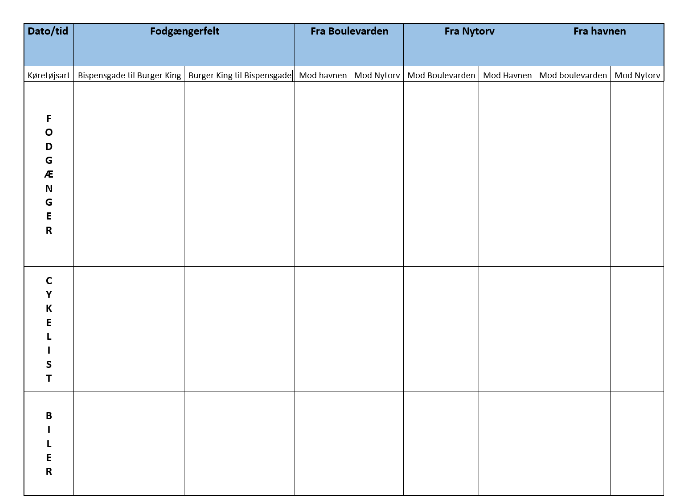
\includegraphics[scale=0.6]{figures/Billederogfigur/tabelp.png}
     \end{adjustbox}
      \caption{Tælleskema for trafiktællinger}
      \label{fig:tft}
    \end{figure}

\end{document}
